% Created 2016-01-08 Fri 16:42
\documentclass[presentation]{beamer}
\usepackage[utf8]{inputenc}
\usepackage[T1]{fontenc}
\usepackage{fixltx2e}
\usepackage{graphicx}
\usepackage{grffile}
\usepackage{longtable}
\usepackage{wrapfig}
\usepackage{rotating}
\usepackage[normalem]{ulem}
\usepackage{amsmath}
\usepackage{textcomp}
\usepackage{amssymb}
\usepackage{capt-of}
\usepackage{hyperref}
\usepackage{minted}
\usepackage{tikz}
\usepgflibrary{shapes.geometric}
\usetikzlibrary{calc}
\usetikzlibrary{positioning}
\usetheme{EPCC}
\author{Lawrence Mitchell\thanks{lawrence.mitchell@ed.ac.uk} (EPCC), Florian Rathgeber, Graham Markall, Nicolas Loriant, Carlo Bertolli, David Ham, Paul Kelly (Imperial College), Gihan Mudalige, Mike Giles (Oxford)}
\date{Tuesday 18th March 2013}
\title{PyOP2: a framework for fast, unstructured mesh computations}
\hypersetup{
 pdfauthor={Lawrence Mitchell\thanks{lawrence.mitchell@ed.ac.uk} (EPCC), Florian Rathgeber, Graham Markall, Nicolas Loriant, Carlo Bertolli, David Ham, Paul Kelly (Imperial College), Gihan Mudalige, Mike Giles (Oxford)},
 pdftitle={PyOP2: a framework for fast, unstructured mesh computations},
 pdfkeywords={},
 pdfsubject={},
 pdfcreator={Emacs 24.5.1 (Org mode 8.3.2)}, 
 pdflang={English}}
\begin{document}

\maketitle
\begin{frame}{Outline}
\tableofcontents
\end{frame}


\section{Overview}
\label{sec:orgheadline5}

\begin{frame}[label={sec:orgheadline1}]{Hardware zoo}
\begin{itemize}
\item Multicore CPU
\item Manycore CPU (phi)
\item GPU
\item All tied together with a network
\end{itemize}
\end{frame}

\begin{frame}[label={sec:orgheadline2}]{Performance portability}
\begin{itemize}
\item What if we want our code to run on different hardware?
\item Can we avoid porting to new hardware?
\end{itemize}
\end{frame}

\begin{frame}[label={sec:orgheadline3}]{Premise}
\begin{itemize}
\item Current typical codes intimately tie numerics to implementation
\begin{itemize}
\item Developers must be experts in multiple domains
\end{itemize}
\item Can we design abstractions that separate numerics from
implementation?
\begin{itemize}
\item and allow us to automatically \emph{generate} high-performance code
\end{itemize}
\item Not an auto-parallelising compiler (too much work)
\end{itemize}
\end{frame}

\begin{frame}[label={sec:orgheadline4}]{Problem domain}
\begin{itemize}
\item unstructured mesh computations
\item typically have some elementary operation we wish to apply over all
entities in a mesh
\end{itemize}
\end{frame}

\section{The OP2 abstraction}
\label{sec:orgheadline13}
\begin{frame}[label={sec:orgheadline6}]{Data types}
\begin{itemize}
\item \emph{Sets} of mesh entities
\begin{itemize}
\item vertices
\item facets
\item elements
\item degrees of freedom
\item \ldots{}
\end{itemize}
\end{itemize}

\begin{center}
\only<1>{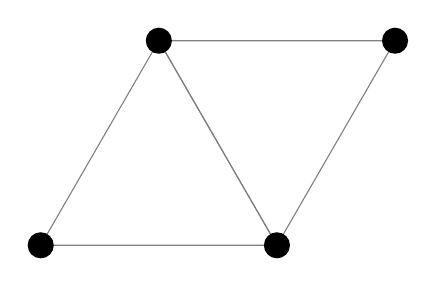
\begin{tikzpicture}[
  mesh/.style={gray},
  vertex/.style={circle, black, fill}]

\draw[mesh] (0,0) -- ++(60:3) -- +(-60:3) -- cycle;
\draw[mesh] (3,0) -- ++(60:3) -- +(-180:3) -- cycle;
\node[vertex] (v1) at (0,0) {};
\node[vertex] (v2) at (60:3) {};
\node[vertex] (v3) at (0:3) {};
\node[vertex] (v4) at ($(0:3) + (60:3)$) {};
\end{tikzpicture}
}

\only<2>{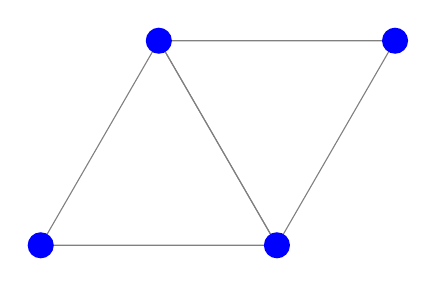
\begin{tikzpicture}[
  mesh/.style={gray},
  vertex/.style={circle, blue, fill}]

\draw[mesh] (0,0) -- ++(60:3) -- +(-60:3) -- cycle;
\draw[mesh] (3,0) -- ++(60:3) -- +(-180:3) -- cycle;
\node[vertex] (v1) at (0,0) {};
\node[vertex] (v2) at (60:3) {};
\node[vertex] (v3) at (0:3) {};
\node[vertex] (v4) at ($(0:3) + (60:3)$) {};
\end{tikzpicture}
}

\only<3>{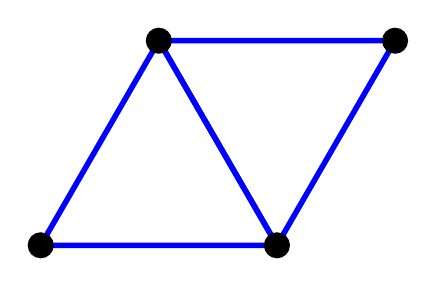
\begin{tikzpicture}[
  mesh/.style={gray},
  vertex/.style={circle, black, fill},
  facet/.style={blue, line width=2pt}]

\draw[mesh, facet] (0,0) -- ++(60:3) -- +(-60:3) -- cycle;
\draw[mesh, facet] (3,0) -- ++(60:3) -- +(-180:3) -- cycle;
\node[vertex] (v1) at (0,0) {};
\node[vertex] (v2) at (60:3) {};
\node[vertex] (v3) at (0:3) {};
\node[vertex] (v4) at ($(0:3) + (60:3)$) {};
\end{tikzpicture}
}

\only<4>{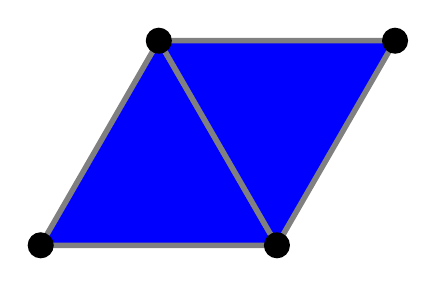
\begin{tikzpicture}[
  mesh/.style={gray, line width=2, fill=blue},
  vertex/.style={circle, black, fill}]

\draw[mesh] (0,0) -- ++(60:3) -- +(-60:3) -- cycle;
\draw[mesh] (3,0) -- ++(60:3) -- +(-180:3) -- cycle;
\node[vertex] (v1) at (0,0) {};
\node[vertex] (v2) at (60:3) {};
\node[vertex] (v3) at (0:3) {};
\node[vertex] (v4) at ($(0:3) + (60:3)$) {};
\end{tikzpicture}
}

\only<5>{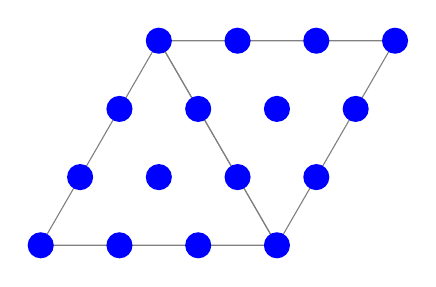
\begin{tikzpicture}[
  dof/.style={circle, blue, fill},
  mesh/.style={gray},
  vertex/.style={circle, blue, fill}]

\draw[mesh] (0,0) -- ++(60:3) -- +(-60:3) -- cycle;
\draw[mesh] (3,0) -- ++(60:3) -- +(-180:3) -- cycle;
\node[vertex] (v1) at (0,0) {};
\node[vertex] (v2) at (60:3) {};
\node[vertex] (v3) at (0:3) {};
\node[vertex] (v4) at ($(0:3) + (60:3)$) {};
\node[dof] (fd1) at (0:1) {};
\node[dof] (fd2) at (0:2) {};
\node[dof] (fd3) at (60:1) {};
\node[dof] (fd4) at (60:2) {};
\node[dof] (fd5) at ($(0:3) + (120:1)$) {};
\node[dof] (fd6) at ($(0:3) + (120:2)$) {};
\node[dof] (fd7) at ($(0:3) + (60:1)$) {};
\node[dof] (fd8) at ($(0:3) + (60:2)$) {};
\node[dof] (fd9) at ($(60:3) + (0:1)$) {};
\node[dof] (fd10) at ($(60:3) + (0:2)$) {};
\node[dof] (ed1) at (intersection cs: 
first line={(0,0)--(30:3)}, 
second line={(0:3)--($(0:3) + (150:3)$)}) {};
\node[dof] (ed2) at (intersection cs: 
first line={(0:3)--($(0:3) + (90:3)$)}, 
second line={(60:3)--($(60:3) + (-30:3)$)}) {};
\end{tikzpicture}
}
\par
\end{center}
\end{frame}

\begin{frame}[label={sec:orgheadline7}]{Data types II}
\begin{itemize}
\item \emph{Maps} between \emph{Sets}
\begin{itemize}
\item e.g. from elements to degrees of freedom
\end{itemize}
\item \emph{Dats}: data defined on a \emph{Set}
\item \emph{Kernels}
\begin{itemize}
\item code snippets to apply pointwise across \emph{Sets}
\end{itemize}
\item \emph{Sparsities} composed of outer products of pairs of \emph{Maps}
\begin{itemize}
\item give positions of non-zeros in discretisation of your operator
\end{itemize}
\item \emph{Mats}: data defined on a \emph{Sparsity}
\end{itemize}
\end{frame}

\begin{frame}[label={sec:orgheadline8}]{Iteration construct}
\begin{itemize}
\item \emph{par$\backslash$\(_{\text{loop}}\)}
\begin{itemize}
\item apply a \emph{Kernel} over every element in a \emph{Set}
\item access data in \emph{Dats} directly, or indirectly through \emph{Maps}
\end{itemize}
\item explicit access descriptors
\begin{itemize}
\item determination of concurrent writes, need for halo swaps can be
made by (simple) code
\end{itemize}
\end{itemize}
\end{frame}

\begin{frame}[label={sec:orgheadline9}]{Code generation targets}
\begin{itemize}
\item C (+ OpenMP) + MPI
\item CUDA (+ MPI [matrices not supported])
\item OpenCL (+ MPI [matrices not supported])
\end{itemize}
\end{frame}

\begin{frame}[fragile,label={sec:orgheadline10}]{Example application code}
 \begin{center}
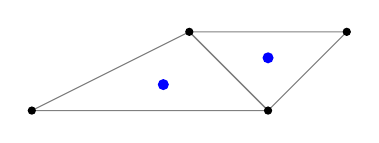
\begin{tikzpicture}[
  mesh/.style={gray},
  vertex/.style={circle, black, fill, inner sep=0pt, minimum size = 3pt},
centroid/.style={circle, blue, fill, inner sep=0pt, minimum size = 4pt}]

\draw[mesh] (0,0) -- (3,0) -- (2,1) -- cycle;
\draw[mesh] (3,0) -- (4,1) -- (2,1) -- cycle;
\node[vertex] (v1) at (0,0) {};
\node[vertex] (v2) at (3,0) {};
\node[vertex] (v3) at (2,1) {};
\node[vertex] (v4) at (4,1) {};

\node[centroid] (c1) at (1.67, 0.33) {};
\node[centroid] (c2) at (3, 0.67) {};
\end{tikzpicture}

\end{center}
\begin{minted}[frame=none,xleftmargin=1em,xrightmargin=1em,fontsize=\scriptsize,mathescape]{python}
vertices = Set(4)
cells = Set(2)
cell2vertex = Map(cells, vertices, 3, [0, 1, 2, 1, 2, 3])
coords = Dat(vertices, 2, [[0, 0], [3, 0], [2, 1], [4, 1]])
centroids = Dat(cells, 2, [[0, 0], [0, 0]])
centroid = Kernel("""void centroid(double *out, double *in[2]) {
        out[0] = (1.0/3.0) * (in[0][0] + in[1][0] + in[2][0]);
        out[1] = (1.0/3.0) * (in[0][1] + in[1][1] + in[2][1]);
                     }""", "centroid")
par_loop(centroid, cells, centroids(IdentityMap, WRITE),
         coords(cell2vertex, READ))
\end{minted}
\end{frame}

\begin{frame}[label={sec:orgheadline11}]{What happens under the hood}
\begin{itemize}
\item data structures recorded
\item par$\backslash$\(_{\text{loop}}\) encountered
\begin{itemize}
\item appropriate backend-specific code generated (cached for later use)
\item \ldots{} and executed
\item if necessary:
\begin{itemize}
\item MPI halo swaps performed
\item data uploaded to accelerator device
\end{itemize}
\end{itemize}
\end{itemize}
\end{frame}

\begin{frame}[label={sec:orgheadline12}]{Picture}
\begin{center}
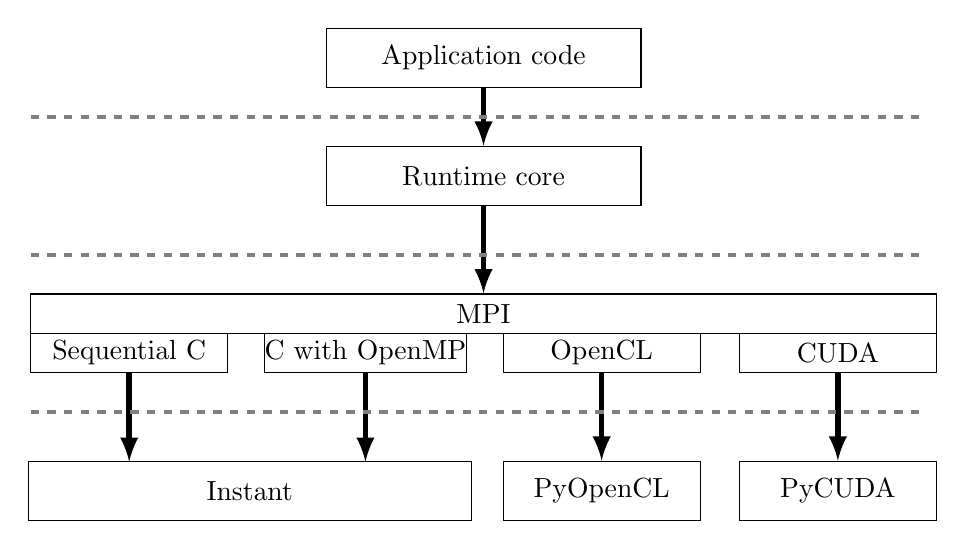
\begin{tikzpicture}[terminal/.style={draw, rectangle, 
 inner sep = 0pt, rounded corners=0mm, minimum height=0.75cm},
arrow/.style={-latex, draw, line width=2pt, black},
sep/.style={dashed, line width=1.5pt, gray}]


\node (user) at (0,0) [terminal, minimum width=4cm] {Application code};
\node (rt) at (0, -1.5) [terminal, minimum width=4cm] {Runtime core};

\node (mpi) at (0, -3.25) [terminal, minimum width=11.5cm, minimum height=0.5cm] {MPI};
\node (sc) at (-4.5, -3.75) [terminal, minimum width=2.5cm, minimum height=0.5cm] {Sequential C};
\node (oc) at (-1.5, -3.75) [terminal, minimum width=2.5cm, minimum height=0.5cm] {C with OpenMP};

\node (cl) at (1.5, -3.75) [terminal, minimum width=2.5cm, minimum height=0.5cm] {OpenCL};
\node (cu) at (4.5, -3.75) [terminal, minimum width=2.5cm, minimum height=0.5cm] {CUDA};

\node (instant) at (-2.97, -5.5) [terminal, minimum width=5.625cm] {Instant};
\node (pycl) at (1.5, -5.5) [terminal, minimum width=2.5cm] {PyOpenCL};
\node (pycu) at (4.5, -5.5) [terminal, minimum width=2.5cm] {PyCUDA};

\draw[arrow] (user) -- (rt);
\draw[arrow] (rt.south) -- (mpi.north);
% \draw[arrow] (rt.south) -- (cl.north);
% \draw[arrow] (rt.south) -- (cu.north);
\draw[arrow] (sc.south) -- +(0, -1.125);
\draw[arrow] (oc.south) -- +(0, -1.125);
\draw[arrow] (cl) -- (pycl);
\draw[arrow] (cu) -- (pycu);

\draw[sep] (-5.75, -0.75) -- (5.625, -0.75);
\draw[sep] (-5.75, -2.5) -- (5.625, -2.5);
\draw[sep] (-5.75, -4.5) -- (5.625, -4.5);

\end{tikzpicture}

\end{center}
\end{frame}

\section{Separating intent from implementation}
\label{sec:orgheadline20}

\begin{frame}[label={sec:orgheadline14}]{User/Runtime requirements}
\begin{itemize}
\item User defines
\begin{itemize}
\item execution, but not order
\item data (with specified input layout)
\item data access (isn't allowed to lie, otherwise they'll get
incorrect results)
\end{itemize}

\item Runtime library can
\begin{itemize}
\item choose to execute iteration in any order
\item choose to rearrange data (e.g. SoA vs. AoS)
\item split/fuse/reorder par$\backslash$\(_{\text{loops}}\)
\item as long as the result is correct
\end{itemize}
\end{itemize}
\end{frame}

\begin{frame}[label={sec:orgheadline15}]{As a result \ldots{}}
\begin{itemize}
\item we can rearrange data to be SoA on GPUs
\begin{itemize}
\item better memory coalescing
\end{itemize}
\item we can fuse user kernels (this is ``easy'' because we have explicit
data dependencies)
\item we can choose different representations of matrices
\begin{itemize}
\item e.g. fully or partially assembled, or matrix free [Markall
et al 2012 \url{doi:10.1002/fld.3648}]
\end{itemize}
\item \ldots{}
\end{itemize}
\end{frame}

\begin{frame}[label={sec:orgheadline16}]{\ldots{}}
\begin{itemize}
\item On GPUs, we explicitly manage shared memory cache
\item For shared memory parallelism (GPU + OpenMP on CPU)
\begin{itemize}
\item we can determine data dependencies and avoid race conditions
\item cache block if appropriate
\end{itemize}
\item Determine when halo swaps are required on distributed memory
systems
\end{itemize}
\end{frame}

\begin{frame}[label={sec:orgheadline17}]{Performance}
\begin{itemize}
\item Runtime library used to replace FE advection-diffusion solver in
Fluidity's dynamical core
\begin{itemize}
\item use FEniCS code generation technology for elementary kernel
\end{itemize}
\item Code runs faster in serial (maintains advantage in MPI parallel)
\item Taking advantage of GPUs: one line change in source code.
\end{itemize}
\end{frame}

\begin{frame}[label={sec:orgheadline18}]{Test case}
\begin{itemize}
\item 2D Advection-diffusion, P1 Lagrange elements, 100 timesteps
\item Compare Fluidity builtin support with PyOP2 on various backends
\item CPU: 12 core Westmere; GPU: C2050
\end{itemize}
\begin{center}
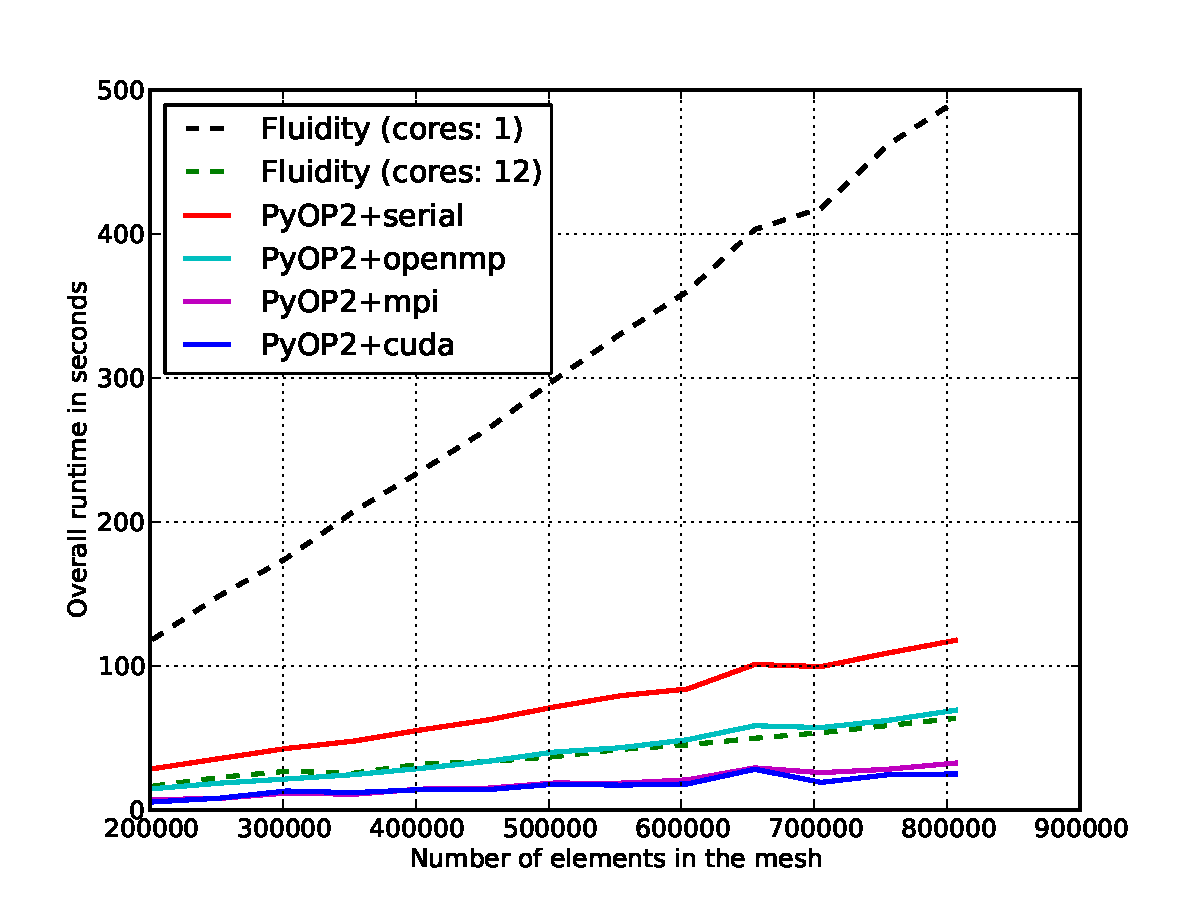
\includegraphics[height=0.7\textheight]{04-11-EASC-PyOP2-fluidity.figures/runtime_linear}
\end{center}
\end{frame}

\begin{frame}[fragile,label={sec:orgheadline19}]{How much code?}
 \begin{itemize}
\item Fluidity
\end{itemize}
\begin{minted}[frame=none,xleftmargin=1em,xrightmargin=1em,fontsize=\scriptsize,mathescape]{fortran}
1500 lines of fortran elided
\end{minted}
\begin{itemize}
\item PyOP2 (using FEniCS to generate kernel code)
\end{itemize}
\begin{minted}[frame=none,xleftmargin=1em,xrightmargin=1em,fontsize=\scriptsize,mathescape]{python}
t = state.scalar_fields["Tracer"]
u = state.vector_fields["Velocity"]
p = TrialFunction(t)
q = TestFunction(t)
diffusivity = 0.1
M = p*q*dx
d = dt*(diffusivity*dot(grad(q),grad(p)) - dot(grad(q),u)*p)*dx
a = M + 0.5*d
L = action(M - 0.5*d, t)
solve(a == L, t)
\end{minted}
\end{frame}
\section{Conclusions}
\label{sec:orgheadline24}

\begin{frame}[label={sec:orgheadline21}]{Conclusions}
\begin{itemize}
\item Given a suitably constrained domain
\begin{itemize}
\item it's possible to automatically generate performance-portable code
\end{itemize}
\item many optimisations possible that would be incredibly difficult to do
by hand (and if possible, highly unmaintainable)
\item writing code is less error-prone
\item your application code is better able to cope with changing hardware
\end{itemize}
\end{frame}

\begin{frame}[label={sec:orgheadline22}]{Future work}
\begin{itemize}
\item Matrix-free application of FE operators
\scriptsize [Kirby and Kieu, Numerische Mathematik 121(2):261 (2012), Ainsworth
et al SIAM JSC 33(6):3087 (2011)]
\begin{itemize}
\item turns sparse LA into application of dense
blocks + gather/scatter
\end{itemize}

\item Lazy evaluation (e.g. postponing halo swap completion as late as possible)

\item 2d unstructured + 1d structured (for ocean/climate)
\begin{itemize}
\item currently under development at IC
\end{itemize}
\end{itemize}
\end{frame}

\begin{frame}[label={sec:orgheadline23}]{Thanks}
\begin{itemize}
\item Code is available (BSD license)
\begin{itemize}
\item \url{http://github.com/OP2/PyOP2}
\item \url{http://www.oerc.ox.ac.uk/research/op2}
\end{itemize}
\item Funding
\begin{itemize}
\item MAPDES (EPSRC grants EP/I00677X/1, EP/I006079/1)
\item APOS-EU (EU FP7/277481)
\end{itemize}
\end{itemize}
\end{frame}
\end{document}
